\chapter{Noosfero}
\label{cap:noosfero}

Nesse capítulo discutimos os benefícios da utilização de uma
plataforma de software livre, bem como, apresentamos a plataforma para criação de
redes sociais livres Noosfero.
%
Escolhemos trabalhar com software livre por
entendermos que este é um integrante fundamental no ensino da ciência e 
tecnologia, estando alinhado à ideologia de livre compartilhamento de
conhecimento~\cite{kon2011}.
%
Outro fator para a utilização de software livre é o
fato de não termos que nos comprometermos a assinar um termo de compromisso
restritivo em redes sociais proprietárias, que, em geral, possuem cláusula que dão à
empresa proprietária a propriedade intelectual em cima de todo o conteúdo
gerado nela.


\section{Software Livre}

Extraído da tese de doutorado de \citeonline{meirelles2013}, discutiremos os
principais ponto relacionados ao o que é software livre do ponto de vista legal e
das vantagens do desenvolvimento colaborativo.
%
Primeiramente, o que define e diferencia
o software livre do que podemos denominar de software restrito passa pelo
entendimento desses quatro pontos dentro do que é
conhecido como o \textit{ecossistema do software livre}.
%
O princípio básico desse ecossistema é promover a liberdade do usuário,
sem discriminar quem tem permissão para usar um software e seus limites de uso,
baseado na colaboração e num processo de desenvolvimento aberto.
%
Software livre é aquele que permite aos usuários usá-lo, estudá-lo, modificá-lo e
redistribui-lo, em geral, sem restrições para tal e prevenindo que não sejam
impostas restrições aos futuros usuários. 
%
Mais precisamente, o software livre garante quatro direitos a seus usuários
~\footnote{Extraído de \url{http://www.gnu.org/} em Dezembro de 2013}:

\begin{itemize}
  \item A liberdade de utilizar o software, para qualquer propósito;
  \item A liberdade de estudar como o software funciona e adaptá-lo para suas necessidades;
  \item A liberdade de redistribuir cópias para seus vizinhos;
  \item A liberdade de aprimorar o software, e redistribuir seus aprimoramentos para o público,
  de forma a beneficiar toda a comunidade;
\end{itemize}

Outro ponto é que esse software existe por meio de projetos de desenvolvimento
que estão centradas em torno de algum código-fonte acessível ao público,
geralmente em um repositório na Internet, onde desenvolvedores e usuários
podem interagir.
%
O código é necessariamente licenciado sob termos legais formais que estão de
acordo com as definições da \textit{Free Software Foundation}
\footnote{\url{http://www.gnu.org/philosophy/free-sw.html}} ou da
\textit{Open Source Initiative}
\footnote{\url{http://www.opensource.org/docs/definition.html}}.

%------------------------------------------------------------------------------%

Uma vantagem oferecida pelo software livre em comparação ao software
restrito vem do fato de que o código-fonte pode ser livremente compartilhado.
%
Esse compartilhamento pode simplificar o desenvolvimento de aplicações
personalizadas, que não precisam ser programadas a partir do zero, mas
podem basear-se em soluções já existentes.

Outra vantagem resultante do compartilhamento do código se refere
à possível melhoria na qualidade, em particular frente aos
problemas inerentes à sua complexidade \cite{CatedralBazzar}.
%
Isso se deve ao maior número de desenvolvedores e usuários envolvidos
com o software. Em outras palavras, um número maior de desenvolvedores, com diferentes
perspectivas e necessidades, é capaz de identificar melhorias e corrigir
mais \emph{bugs} em menos tempo e, consequentemente, promover refatorações que,
geralmente, levam à melhoria do código.
%
Além disso, um número maior de usuários gera situações de uso e
necessidades mais variadas, o que se traduz em um maior número
de \emph{bugs} identificados e mais sugestões de melhorias.

%------------------------------------------------------------------------------%

\section{Noosfero, Uma Plataforma Livre para Redes Sociais}
\label{noosfero-section}

Noosfero~\footnote{\url{http://www.noosfero.org}}
é uma  plataforma web livre para criação de redes sociais, desenvolvida
pela Cooperativa de Tecnologias Livres - Colivre
~\footnote{\url{http://www.colivre.coop.br}},
em 2007, sob licença AGPL v.3, com a proposta de permitir aos usuários criarem sua
própria rede social personalizada, livre e autônoma.

%------------------------------------------------------------------------------%

O Noosfero foi desenvolvido na linguagem de programação Ruby
~\footnote{\url{http://www.ruby-lang.org/en/}},
versão 1.8.7, e utiliza o \textit{framework} Model-View-Controller (MVC) para aplicações web Ruby on Rails
~\footnote{\url{http://rubyonrails.org/}}, versão 2.3.5.
%
A escolha destas tecnologias, por parte dos criadores do Noosfero, que também
trabalhamos juntos no contexto deste trabalho,
foi baseada no fato de que o Ruby possui uma sintaxe
simples, elegante e de fácil leitura, o que aumenta a manutenibilidade do sistema,
uma característica importante num projeto de software livre que visa atrair
desenvolvedores externos~\cite{meirelles2013}. 
%
Outras características importantes que influenciaram essa escolha são a alta
capacidade produtiva que o \textit{framework} possui por priorizar conceitos como
\textit{convention over configuration} (convenção antes de configuração)
e DRY~\footnote{Uma forma de apologia ao reuso de código}
(\textit{Don't Repeat Yourself} - Não Repita a Si Mesmo), bem como, o alinhamento
entre a comunidade do Ruby on Rails com metodologias ágeis de
desenvolvimento de software, que são evidenciadas em uma série de ferramentas que
viabilizam o uso de práticas como TDD~\footnote{Desenvolvimento orientado a testes}
e BDD~\footnote{Design orientado a comportamento}, práticas adotadas no
desenvolvimento do Noosfero, e neste trabalho.

%------------------------------------------------------------------------------%

A segurança também foi uma preocupação na concepção do Noosfero, o que levou os
desenvolvedores a tomar a decisão de homologar a ferramenta apenas para a
versão do Debian~\footnote{\url{http://www.debian.org/}}
\textit{stable}, por este ser reconhecido por passar por rigorosos testes de
segurança e correção de falhas antes de seu lançamento. 
%
Para manter a compatibilidade, as versões do Ruby e do Rails utilizadas no
Noosfero são as versões disponibilizadas nos repositórios do Debian~\footnote{Por exemplo, a falha de segurança no Ruby on Rails descrita em \url{http://news.ycombinator.com/item?id=5035023}, não impactou o Noosfero, uma vez, diferente do Redmine, uma ferramenta de gestão de projeto amplamente utilizada, o primeiro não tem uma cópia do Ruby on Rails dentro do
seu código-fonte, o que é uma prática ruim, por dificultar como lidar com problemas de segurança. O Noosfero utiliza o pacote do Ruby on Rails oficial do Debian, de forma que uma
vez que a vulnerabilidade é corrigida no Debian, não é preciso corrigir no Noosfero. No caso do Redmine, a versão empacotada no Debian também utiliza essa abordagem, que
faz parte da política técnica do Debian, ou seja, não embarcar cópias de bibliotecas, \textit{frameworks} etc.}.

%------------------------------------------------------------------------------%

A arquitetura do Noosfero foi pensada para permitir que este seja facilmente
expansível, de forma que funcionalidades que não sejam comuns ao conceito de
redes sociais sejam desenvolvidos como \textit{plugins}, assim diminuindo
o acoplamento e aumentando a coesão dos diversos módulos do sistema.
%
Uma das grandes vantagens em se criar uma aplicação com arquitetura extensível
é a possibilidade de criar \textit{plugins} sem precisar modificar o código
fonte do núcleo da ferramenta, além de permitir o isolamento de
\textit{bugs} encontrados mais facilmente.

Os mantenedores do Noosfero, responsáveis por aprovar solicitações de
alteração no código, exigem que os \textit{plugins} tenham um certo nível de
testes para que esses possam ser incorporados à uma versão do Noosfero para
evitar a inserção de \textit{bugs} que afetem o \textit{core} ou
outros \textit{plugins}, além de manter o padrão de qualidade de código.

Essa abordagem arquitetural é muito benéfica para a diversidade de contextos
em que o Noosfero pode ser utilizado. Diversidade essa que pode ser evidenciada
quando se observa a existência de uma rede como o Cirandas
~\footnote{\url{https://cirandas.net/}},
uma rede social com o propósito de promover economia solidária através
da troca e venda de produtos e serviços, e o
Stoa, um ambiente virtual para a disseminação de conhecimento em âmbito
acadêmico de forma colaborativa, ambos desenvolvidos utilizando o Noosfero.
%
Dessa forma, os dois ambientes são instâncias do Noosfero que utilizam o seu núcleo comum,
mas diferem no uso de \textit{plugins} com funcionalidades próprias às suas necessidades específicas.
%
Na seção \ref{funcionalidades}, apresentamos algumas funcionalidades que serão
desenvolvidas no formato de \textit{plugins}.

%------------------------------------------------------------------------------%

\begin{figure}[h]
    \centering
    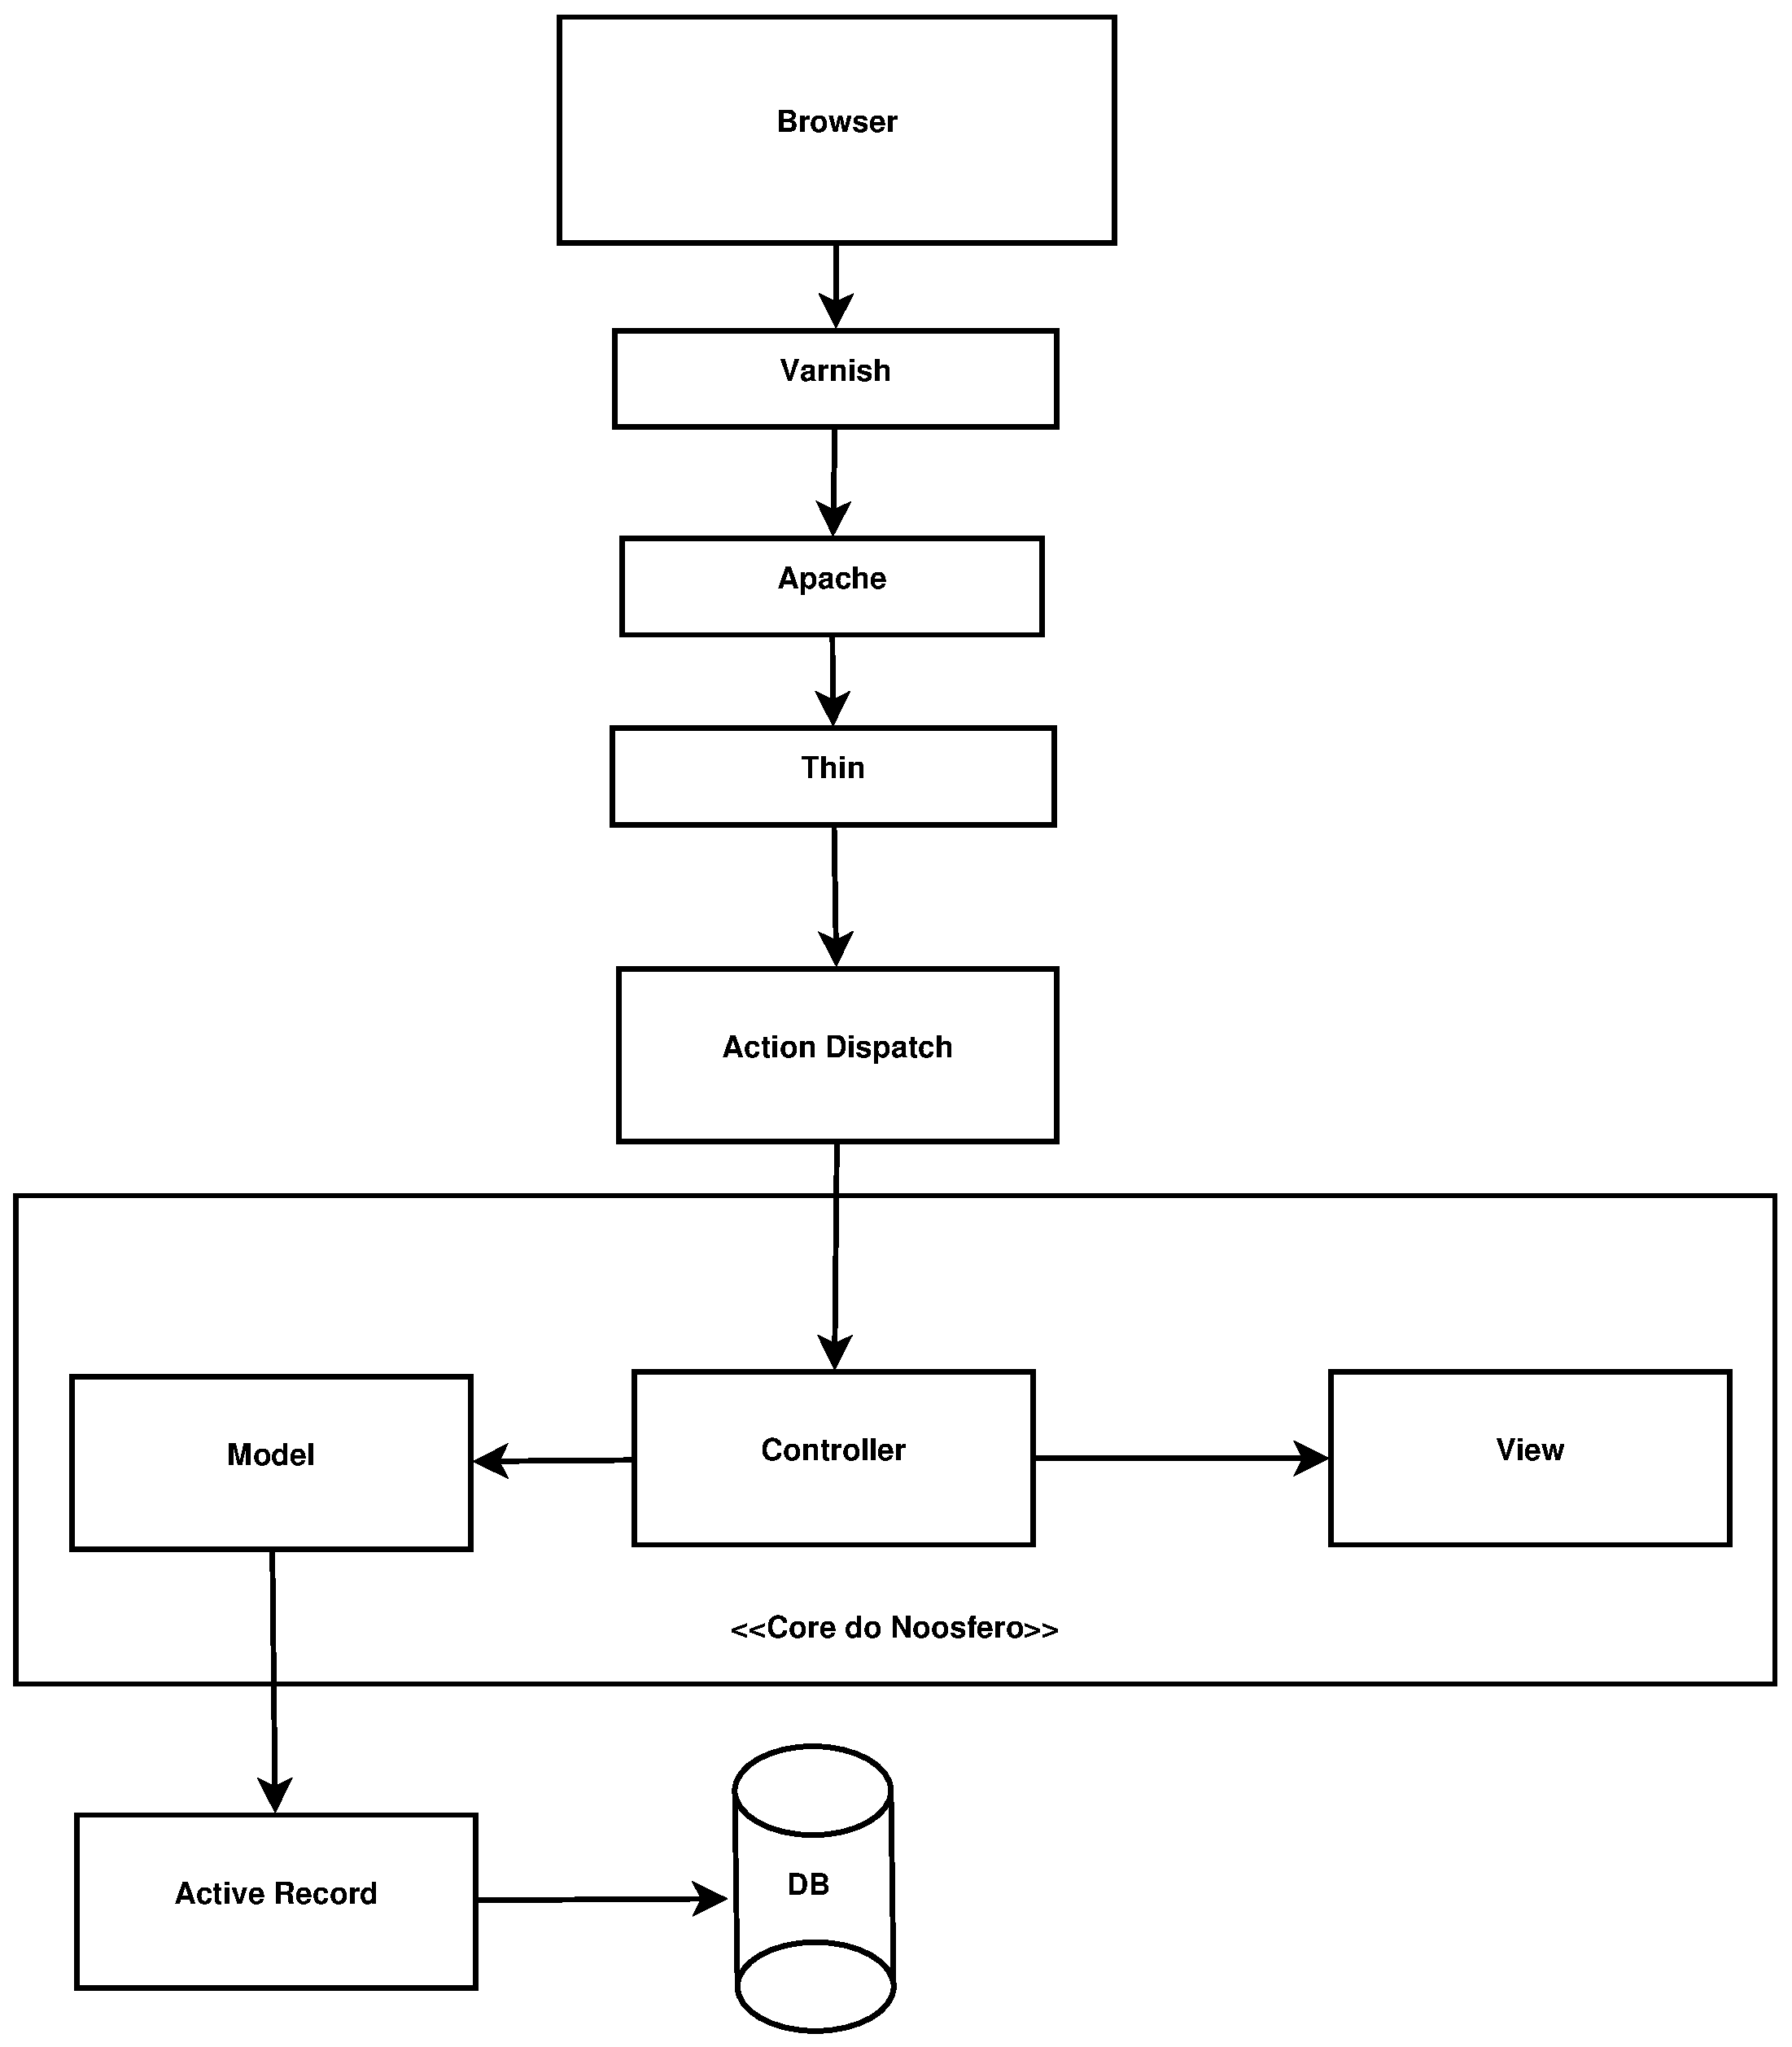
\includegraphics[keepaspectratio=true,scale=0.25]
      {figuras/noosfero_architeture.eps}
    \caption{Visão arquitetural do Noosfero}
    \label{noosfero-arch}
\end{figure}

A Figura \ref{noosfero-arch} apresenta uma visão arquitetural de alto nível
do núcleo do Noosfero. Vale a pena ressaltarmos alguns componentes desta arquitetura:

\begin{itemize}
    \item \textbf{Varnish:} acelerador de aplicações web também conhecido 
    como cache de proxy reverso HTTP. É utilizado quando for necessário
    acessar conteúdo estático, imagens, \textit{scripts} e folhas de estilos.

    \item \textbf{Apache:} \textit{web-server} utilizado como servidor de 
    \textit{proxy} reverso. Sua função é encaminhar as requisições que
    chegam para uma das instâncias do Thin.

    \item \textbf{Thin:} \textit{app-server} utilizado para processar as
    requisições de entrada e saída e encaminhá-las para o Noosfero para que
    ele possa executá-las. Pode ser configurado para utilizar mais de um
    processo para realizar balanceamento de carga. É recomendável o uso de
    dois processos do \textit{Thin} por núcleo de processador do servidor
    hospedeiro.
    
    \item \textbf{ActionDispatch:} funciona como roteador. Sua função é
    mapear as requisições que chegam a suas respectivas \textit{controllers}.
    
    \item \textbf{Controller:} controla o fluxo da aplicação. Realiza a
    ligação entre as entidades de \textit{model} e de \textit{view} através
    de chamadas de métodos.
    
    \item \textbf{Model:} representa as entidades do domínio da aplicação.
    A lógica da aplicação é implementado nas classes de \textit{model}.

    \item \textbf{View:} responsável pela visualização das páginas, isto é,
    as saídas em HTML da aplicação.
    
    \item \textbf{Active Record:} realiza o mapeamento entre os objetos de
    \textit{model} e o modelo relacional utilizado no banco de dados da
    aplicação.        
    
\end{itemize}

%------------------------------------------------------------------------------%

\begin{figure}[h!]
    \centering
    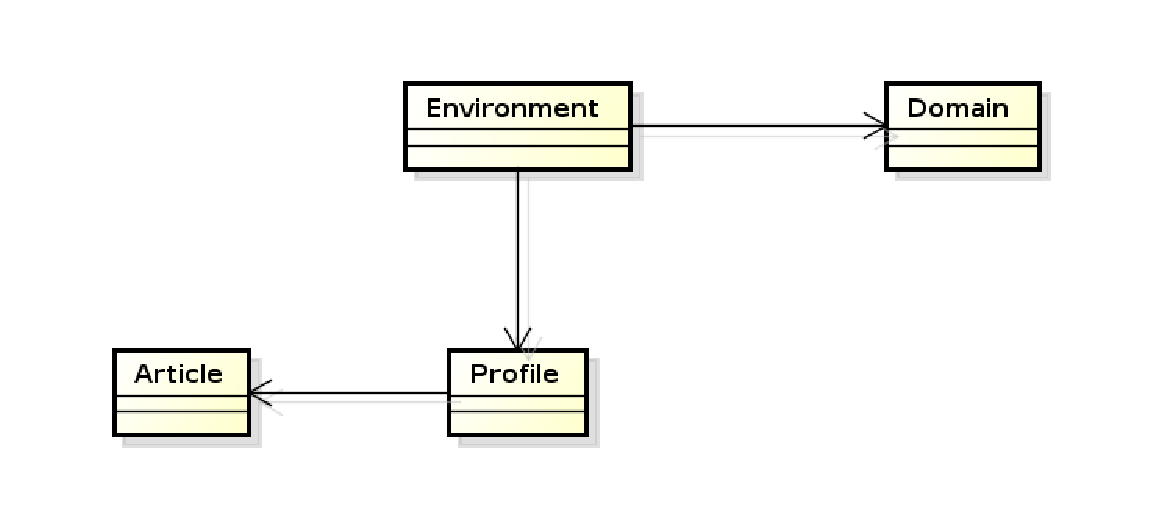
\includegraphics[keepaspectratio=true,scale=0.65]
      {figuras/domain_main.eps}
    \caption{Entidades de domínio: relação entre ambientes, domínios e perfis.}
    \label{domain_main}
\end{figure}

O Noosfero é uma plataforma multi-ambiente, o que significa que se pode ter duas
redes sociais distintas, com domínios, usuários e comunidades distintas em uma
mesma instalação conforme ilustrado na Figura~\ref{domain_main}.
%
A entidade \textbf{\textit{Profile}}, em português \textbf{Perfil}, é uma
abstração das três formas de entidades concretas de perfil existentes no
Noosfero: \textbf{pessoa}, \textbf{comunidade} e \textbf{empreendimento}
(em inglês: \textbf{\textit{person}}, \textbf{\textit{community}} e
\textbf{\textit{enterprise}}).
%
Em outras palavras, as três entidades possuem características em comum e são tratadas
como uma só em determinados contextos dentro da aplicação. Existe ainda
outra entidade que abstraí o comportamento comum à \textbf{comunidades}
e \textbf{empreendimentos} chamada de \textbf{organização} (em inglês,
\textbf{\textit{organization}}).

\begin{figure}[h!]
    \centering
    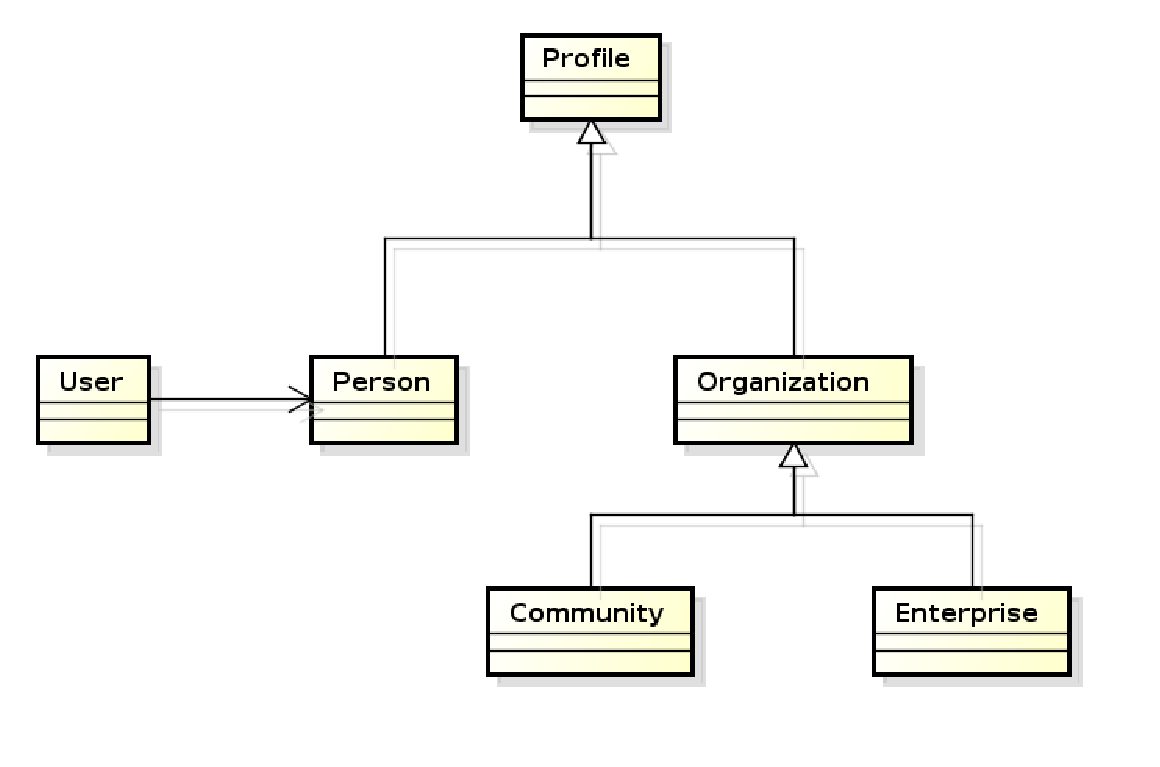
\includegraphics[keepaspectratio=true,scale=0.6]
      {figuras/domain_profiles.eps}
    \caption{Entidades de domínio: tipos de perfis.}
    \label{domain_profiles}
\end{figure}

\begin{figure}[h!]
    \centering
    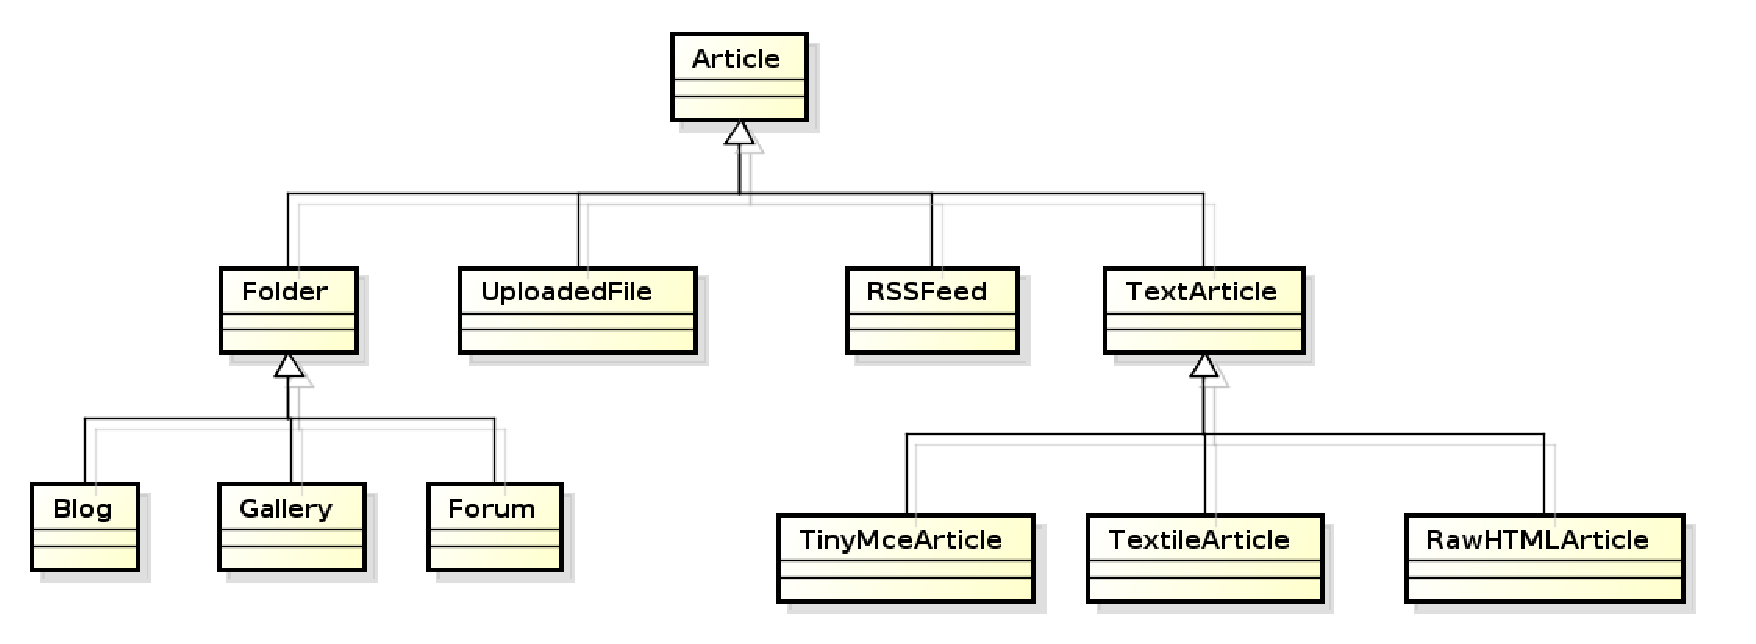
\includegraphics[keepaspectratio=true,scale=0.55]
      {figuras/domain_articles.eps}
    \caption{Entidades de domínio: tipos de artigos.}
    \label{domain_articles}
\end{figure}

A Figura \ref{domain_profiles} apresenta a relação entre os tipos de perfil.
A seta com a cabeça triangular representa uma relação de herança~\footnote{%
\url{http://en.wikipedia.org/wiki/Inheritance_(object-oriented_programming)}}
entre as classes que representam as entidades de domínio.
%
Existe ainda a entidade \textbf{\textit{User}}, ou \textbf{Usuário}, que é
mantida separada da entidade \textbf{Pessoa} por questões de \textit{design}
do código da aplicação, que é quem implementa a lógica de autenticação da
aplicação.
%
Desta forma a lógica de autenticação fica separada da lógica de
visualização e personalização do perfil.
%
Por fim, as entidades mostradas na Figura \ref{domain_articles} representam os
principais tipos de conteúdos disponíveis no Noosfero, \textbf{artigos
de texto}, \textbf{pastas}, \textbf{blogs}, \textbf{galerias de imagens},
\textbf{arquivos} e \textbf{\textit{feeds} de notícias}, assim como a
relação de herança entre estes.

Mesmo com as vantagens do ponto de vista arquitetural e a constante evolução do Noosfero,
essa plataforma ainda necessita de algumas melhorias e novas funcionalidades, que foram
atendidas, em parte, neste trabalho com a implementação e/ou evolução de \textit{plugins}, na
maioria dos casos de nossas colaborações.
%
Também, para avaliarmos a implantação do Noosfero na UnB, prototipamos um \textit{plugins} para autenticação
na base de dados da UnB, de acordo, até o momento, com as autorizações cedidas pelos departamentos responsáveis
~\footnote{As autorizações foram, gentilmente, solicitadas através do CDTC para os órgãos responsáveis por administrar
as diversas bases de dados da UnB, como por exemplo o Decanato de Ensino de Graduação (DEG), responsável pela
base de dados de alunos.} e interações com o Centro de Processamento de Dados (CPD) da instituição. Esses
\textit{plugins} e as demais colaborações, atendendo os requisitos levantados e descritos, serão apresetandos na Seção
~\ref{funcionalidades}, do próximo capítulo.
